\documentclass{article}
\usepackage{url}
\usepackage{listings}
\usepackage{graphicx}


\begin{document}
\lstset{language=bash}
\lstset{basicstyle=\footnotesize,breaklines=true}

\title{A brief guide for AFiVO}
\author{Jannis Teunissen}
\maketitle

\section{Introduction}
\label{sec:introduction}

AFiVO (Adaptive Finite Volume Octree) is a framework that provides the basics
for finite volume simulations with adaptive mesh refinement.
There are already a number of such frameworks available, but afivo is different
in a couple of ways.
For one, it provides less functionality.
This means that there is less code, which should makes it easier to modify
things yourself.

Here are some of other the features of afivo:

\begin{itemize}
  \item Afivo is designed for OpenMP parallelism (shared memory systems).
  \item Afivo comes with a FAS multigrid solver.
  \item Afivo can write VTK output which can be visualized with many tools,
  e.g., Visit.
  \item Afivo supports 2D and 3D meshes.
  \item Afivo is written in \emph{modern} Fortran, and uses some Fortran 2008
  features.
  However, we do not use an object-oriented approach.
\end{itemize}

\section{Quadtree / octree meshes}
\label{sec:amrmesh}

Afivo uses 2:1 balanced quadtree (2D) / octree (3D) meshes, in much the same way
as Paramesh does.
Such meshes can be described by the following rules:

\begin{itemize}
  \item The mesh is constructed from boxes that contain $N^d$ cells, where $d$
  is the number of coordinates.
  \item Boxes can be refined by a factor of two, in which case $2^d$ refined
  boxes are created.
  \item The difference in refinement level for adjacent boxes is at most one.
\end{itemize}

In figure \ref{fig:example-quadtree} you can see some examples of such quadtree
meshes.

\begin{figure}
  \centering
  \includegraphics[width=2.5cm]{figures/quadtree_cex1.png}
  \includegraphics[width=2.5cm]{figures/quadtree_cex2.png}
  \includegraphics[width=2.5cm]{figures/quadtree_cex3.png}
  \includegraphics[width=2.5cm]{figures/quadtree_cex4.png}
  \caption{Examples of a quadtree mesh that gets refined.
    Here boxes contain $2 \times 2$ cells, and different boxes have different
    colours. Note that in the rightmost picture, there are so many boxes that
    differences in colour are hardly visible.}
  \label{fig:example-quadtree}
\end{figure}

\section{Getting and compiling AFiVO}
\label{sec:getting-started}

\subsection{Obtaining the code}
\label{sec:obtaining}

Afivo can be obtained from \url{https://github.com/jannisteunissen/afivo}. If
you have git installed, simply clone the repository like this:

\begin{lstlisting}
  git clone https://github.com/jannisteunissen/afivo
\end{lstlisting}

\subsection{Compiling the code}
\label{sec:compilation}

Compilation requires a relatively new gfortran compiler (ifort is also
supported), and should then be as simple as this:

\begin{lstlisting}
  cd afivo
  make
\end{lstlisting}

This will create a file \texttt{libafivo.a} in the \texttt{src} directory, which
you can link to from your own code.
For that you also need the module files, which are also in the \texttt{src}
directory.
Furthermore, the examples that come with afivo are also compiled, and the
executables can be found in the \texttt{examples} directory.

\lstset{language=[08]Fortran}
\section{Some examples}
\label{sec:examples}


In the \texttt{examples} directory you can find the
examples that come with afivo.
Here we discuss some of them.
The examples produce output in the VTK unstructured format (XML
type\footnote{See \url{http://www.vtk.org/VTK/img/file-formats.pdf} for a
  specification}).
You can visualize these files with for example Visit\footnote{Visit can be
  obtained from \url{https://wci.llnl.gov/simulation/computer-codes/visit}}.

\subsection{Constructing a simple mesh}
\label{sec:example-base}

The first example that we discuss is \texttt{test\_base\_2d.f90}.
There is also a 3D version (\texttt{test\_base\_3d.f90}).

Let us go through the important bits of code.
First, we create a variable \texttt{tree}, which will later contain the complete
mesh with all its data.
Then we need to tell afivo some of the properties of the mesh, to initialize the
\texttt{tree}.

\begin{lstlisting}
  type(a2_t) :: tree

  ! Initialize tree
  call a2_init(tree, & ! Tree to initialize
       box_size, &     ! Number of cells per coordinate in a box
       n_var_cell, &   ! Number of face-centered variables
       n_var_face, &   ! Number of cell-centered variables
       dr)             ! Distance between cells on base level
\end{lstlisting}

For example, in figure \ref{fig:example-quadtree}, \texttt{box\_size} was set to
two. Here we set it to eight.
Now that we have defined the basic properties of a box, let's add two boxes to
the mesh.
We have to define where a box is (a spatial index), and what its neighbors
are.
This is done in the following way
\begin{lstlisting}
  ix_list(:, 1) = [1,1] ! One box at 1,1
  ix_list(:, 2) = [2,1] ! One box at 2,1

  ! Set neighbors for box one
  nb_list(a2_nb_lx, 1) = 2
  nb_list(a2_nb_hx, 1) = 2
  nb_list(a2_nb_ly, 1) = 1
  nb_list(a2_nb_hy, 1) = 1

  ! Set neighbors for box two
  nb_list(:, 2) = 2

  ! Create the base mesh
  call a2_set_base(tree, ix_list, nb_list)
\end{lstlisting}

\begin{figure}
  \centering
  \includegraphics[width=7.5cm]{figures/two_boxes.png}
  \caption{Two boxes of $8 \times 8$ cells, with periodic boundary conditions on
  the outside.}
  \label{fig:two-boxes}
\end{figure}

The result is shown in figure \ref{fig:two-boxes}.
In two dimensions, a spatial index consists of two indices.
See figure \ref{fig:box-indices} for an example.
In afivo, boxes should have positive spatial indices, so (1,1) is the lowest
index you can give.

\begin{figure}
  \centering
  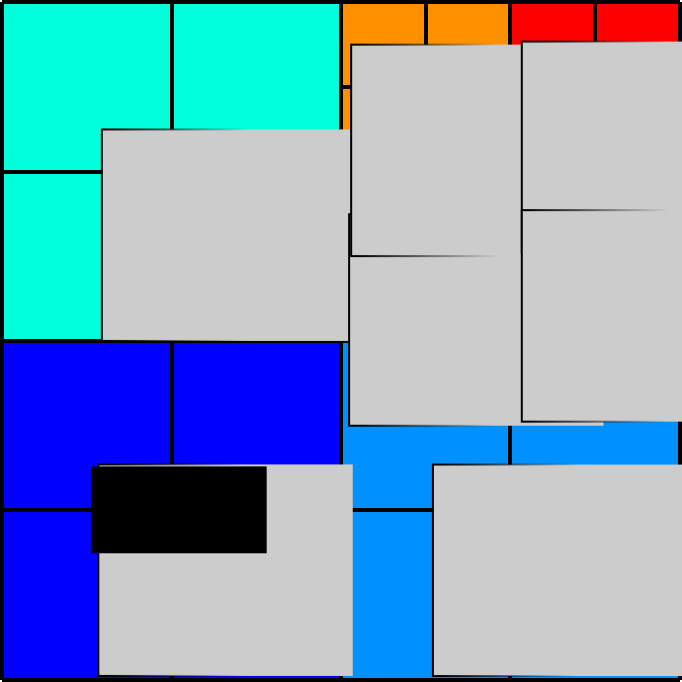
\includegraphics[width=7.5cm]{figures/box_indices.png}
  \caption{An example which shows the spatial indices of boxes that contain
    $2 \times 2$ cells.
    Below the four boxes in the top-right corner lies a (2,2) coarse box.}
  \label{fig:box-indices}
\end{figure}

In two dimensions, a box has four neighbors, which are ordered as lower-x,
higher-x, lower-y, higher-y (and lower-z, higher-z in 3D).
Here we create two boxes next to each other, with periodic boundary conditions.
Note that we do not need to specify all the neighbors for box two, because afivo
is smart enough to understand that if box one has box two has a neighbor, then
that should also be true vice-versa.

\subsection{Refining the mesh}
\label{sec:refining-mesh}

The mesh that we've constructed thus far is shown in figure \ref{fig:two-boxes}.
In order to refine it, we do the following:
\begin{lstlisting}
  call a2_adjust_refinement(tree, ref_func)
\end{lstlisting}

A refinement function gets a box, and can return three values:
\begin{itemize}
  \item \texttt{a5\_kp\_ref} keep refinement as is
  \item \texttt{a5\_do\_ref} refine
  \item \texttt{a5\_rm\_ref} derefine
\end{itemize}
The refinement function in our example is particularly simple, because it
refines or derefines based on a random number:
\begin{lstlisting}
  integer function ref_func(box)
    type(box2_t), intent(in) :: box
    real(dp)                 :: rr

    call random_number(rr)
    if (rr < 0.2_dp .and. box%lvl < 10) then
       ref_func = a5_do_ref
    else
       ref_func = a5_rm_ref
    end if
  end function ref_func
\end{lstlisting}

It is important to understand two things about \texttt{a2\_adjust\_refinement}:
First, it will change the refinement level in some location by at most one.
So sometimes, you will need to call it multiple times.
Second, it will sometimes refine areas that you did not specify for refinement,
to ensure 2:1 balance (no jumps in refinement level).
So the good news is that when you write your refinement function, you do not
need to worry about this.

In figure \ref{fig:random-refinement}, the result is shown after 8 steps of
random refinement.
Note that 2:1 balance is also preserved along the periodic coordinates.

\begin{figure}
  \centering
  \includegraphics[width=7.5cm]{figures/random_ref.png}
  \caption{Random refinement}
  \label{fig:random-refinement}
\end{figure}

\subsection{Working with boxes, levels and trees}
\label{sec:data-structures}

Of course, we do not only want to define a mesh.

\subsection{Filling ghost cells}
\label{sec:ghost-cells}



\end{document}